\documentclass[12pt]{article}
\usepackage[margin=1in]{geometry}
\usepackage{graphicx}
\usepackage[hidelinks]{hyperref}
\usepackage{microtype}
\setlength{\parindent}{0pt}
\setlength{\parskip}{0.6em}
\begin{document}

\begin{center}
{\Large\bfseries Supplementary Information 1}\\[1.2em]
{\large A registered genome-wide analysis identifies robust, context-dependent transcriptional responses of lychee to \textit{Peronophythora litchii}}\\[1.2em]
Eric Zhuang\\
NYU Langone Health, New York, New York, USA
\end{center}

\section*{Contents}

This file contains Figures S1--S3 and their captions. Supplementary Data 2, supplied as \texttt{Discover\_Plants\_Data\_and\_Code.zip}, contains machine-readable Tables S1--S18, all figure source data, the registered protocol and amendment log, analysis code, workflows, configurations, tests, metadata, and environment specifications. The complete archive is also permanently available at \url{https://doi.org/10.5281/zenodo.22436625}.

\begin{itemize}
\item Figure S1: replicate-level normalized counts.
\item Figure S2: conditional parametric power curves.
\item Figure S3: exploratory signed-signature estimate.
\end{itemize}

\clearpage
\setcounter{figure}{0}
\renewcommand{\thefigure}{S\arabic{figure}}

\begin{figure}[p]
\centering
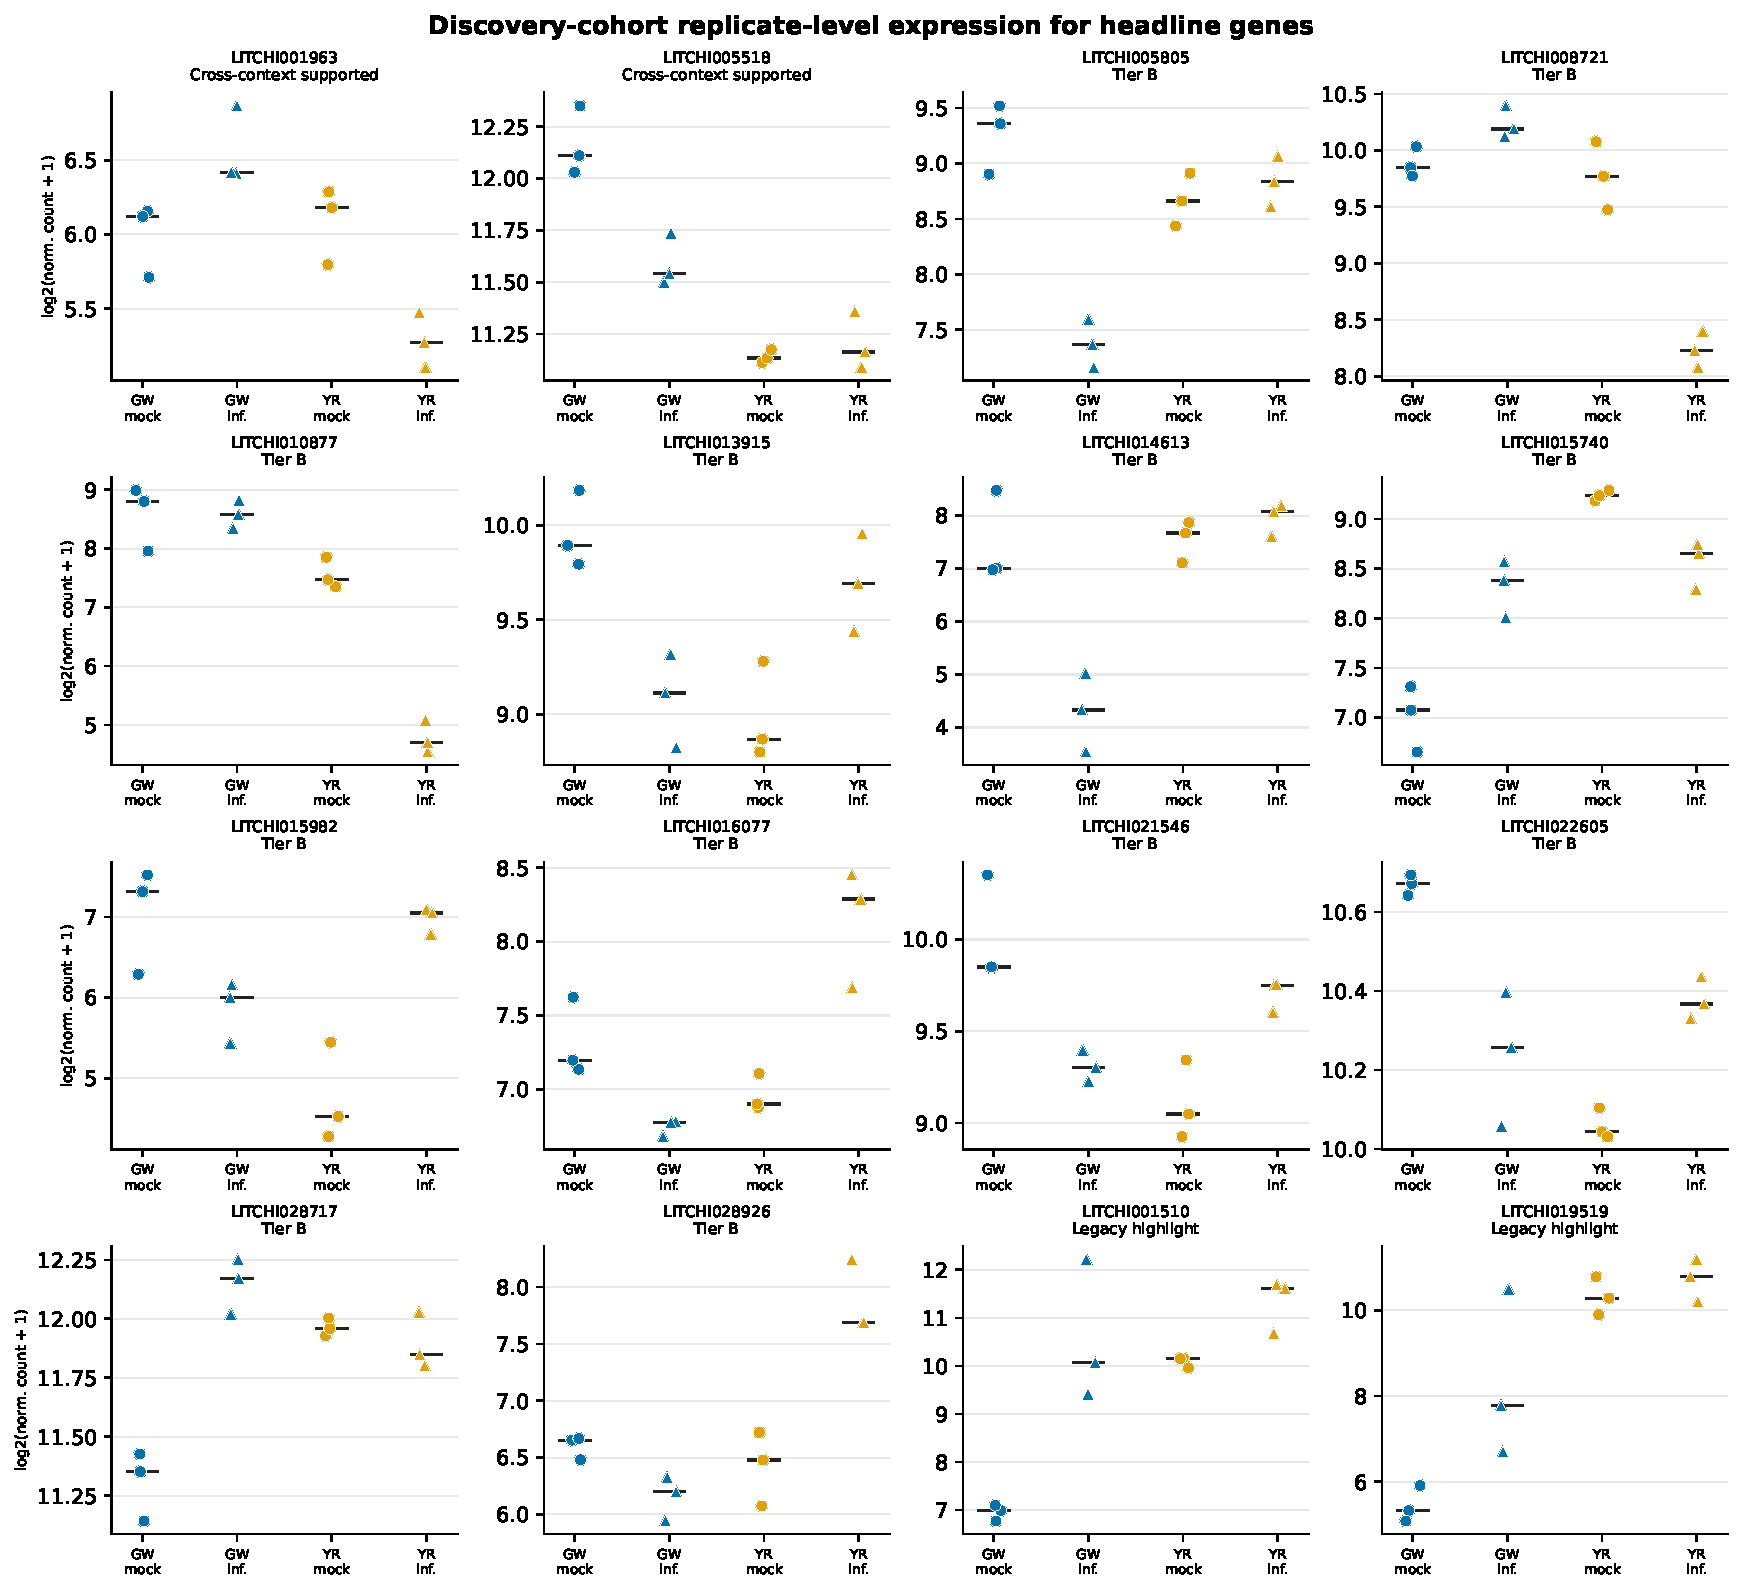
\includegraphics[width=0.96\textwidth,height=0.72\textheight,keepaspectratio]{FigS1.pdf}
\caption{Replicate-level normalized counts for the two cross-context-supported genes, twelve Tier B genes, and two legacy highlights. Points are individual deposited libraries; bars show cultivar-treatment medians.}
\end{figure}
\clearpage

\begin{figure}[p]
\centering
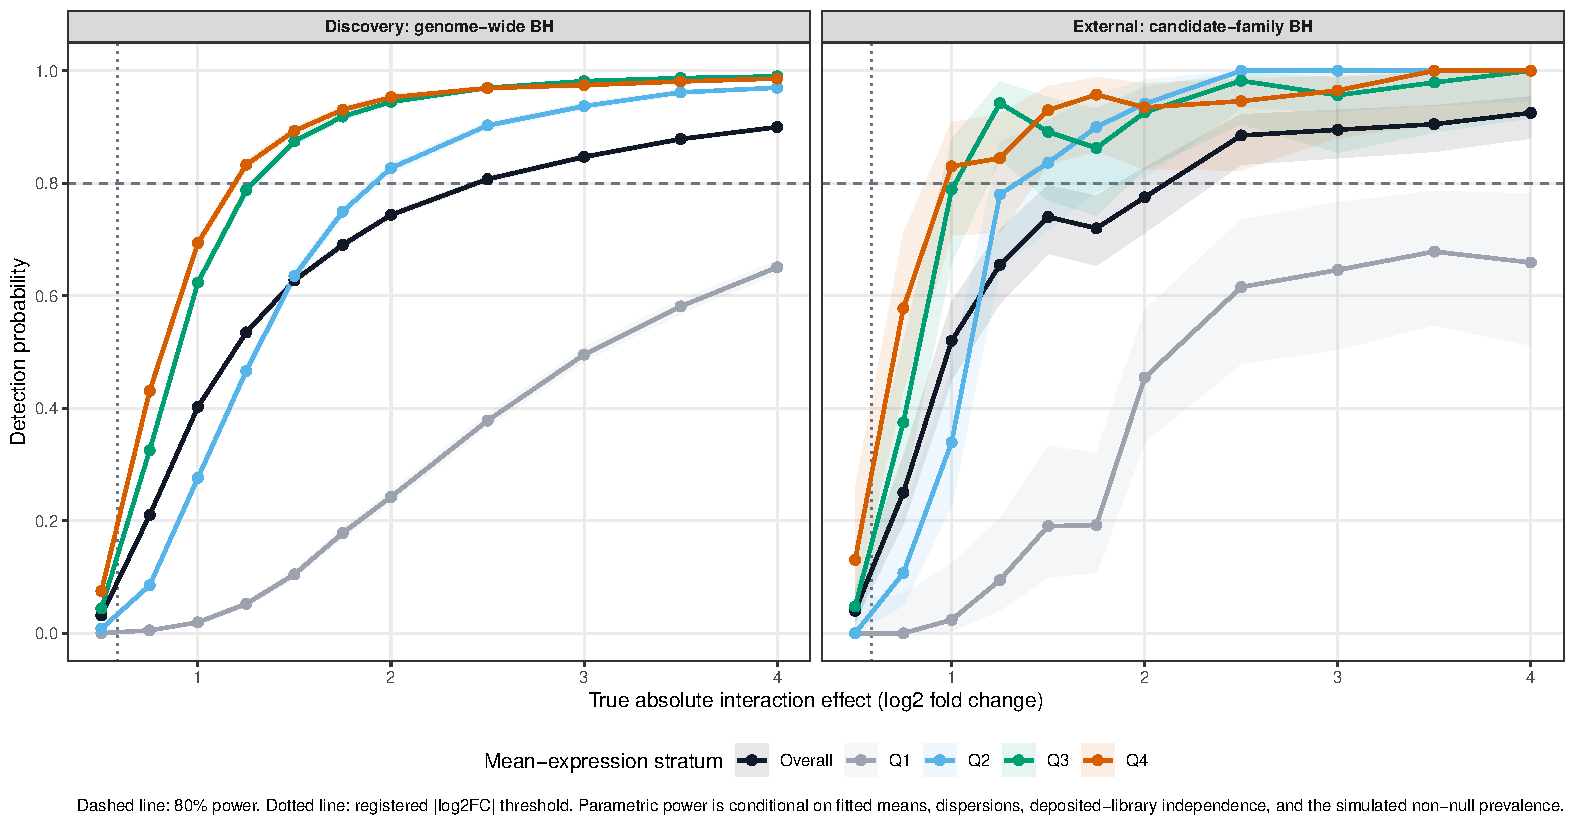
\includegraphics[width=0.96\textwidth,height=0.72\textheight,keepaspectratio]{FigS2.pdf}
\caption{Parametric detection probability for cultivar-by-infection effects under genome-wide discovery and candidate-family external adjustment. Curves show the overall result and mean-expression quartiles; the dashed line marks 80\% power.}
\end{figure}
\clearpage

\begin{figure}[p]
\centering
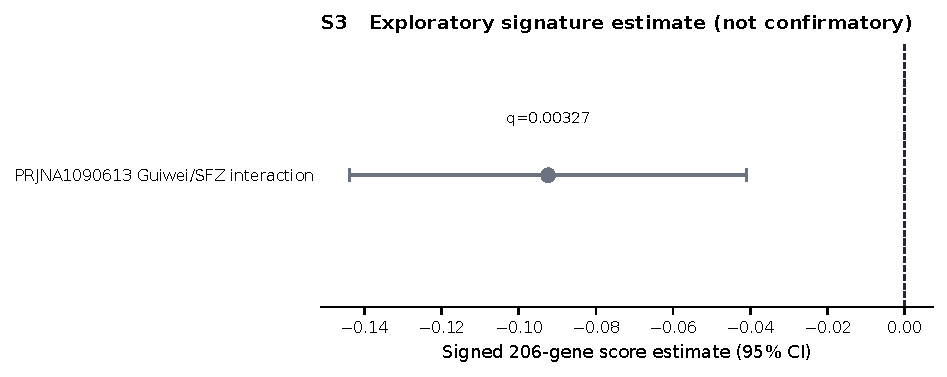
\includegraphics[width=0.96\textwidth,height=0.72\textheight,keepaspectratio]{FigS3.pdf}
\caption{Exploratory PRJNA1090613 signed-signature estimate, shown separately because cohort metadata did not support its inclusion in the confirmatory evaluation.}
\end{figure}
\clearpage

\end{document}
